\documentclass[aspectratio=169]{beamer}

\usepackage[english]{babel}
\usepackage{devedeamer}

\title{Devedeamer}
\subtitle{A simplified beamer template}
\author{David Gomes}
\institute{UFPR}

\begin{document}

\begin{frame}[plain, noframenumbering]    
\titlepage
\end{frame}

\begin{frame}[plain, noframenumbering]{Outline}
\frametitle{Table of Contents}
\tableofcontents[hideallsubsections]
\end{frame}

\section{Enumerate}
\begin{frame}
\frametitle{Enumerate}

There are three important points:
\begin{enumerate}
    \item<1-> A first one,
    \item<2-> a second one with a bunch of subpoints,
        \begin{itemize}
            \item first subpoint. (Only shown from second slide on!).
            \item<3-> second subpoint added on third slide.
                \begin{itemize}
                    \item first subsubpoint.
                    \item<4-> second subsubpoint added on fourth slide.
                \end{itemize}
            \item<5-> third subpoint added on fifth slide.
        \end{itemize}
    \item<6-> and a third one.
\end{enumerate}

\end{frame}

\section{Blocks}
\begin{frame}
\frametitle{Blocks}

\begin{block}{Beamer}
Beamer is a LaTeX document class for creating presentation slides, with a wide range of templates and a set of features for making slideshow effects.
\end{block}

\begin{definition}
Beamer is a LaTeX document class for creating presentation slides, with a wide range of templates and a set of features for making slideshow effects.
\end{definition}

\begin{alertblock}{Danger}
Beamer is a LaTeX document class for creating presentation slides, with a wide range of templates and a set of features for making slideshow effects.
\end{alertblock}

\begin{example}
Beamer is a LaTeX document class for creating presentation slides, with a wide range of templates and a set of features for making slideshow effects.
\end{example}

\end{frame}

\begin{frame}
\frametitle{Blocks}

\begin{theorem}[Pythagoras]
$a^2 = b^2 + c^2$
\end{theorem}

\begin{corollary}
Beamer is a LaTeX document class for creating presentation slides, with a wide range of templates and a set of features for making slideshow effects.
\end{corollary}

\begin{proof}
Beamer is a LaTeX document class for creating presentation slides, with a wide range of templates and a set of features for making slideshow effects.
\end{proof}

\end{frame}

\section{Quote}
\begin{frame}
\frametitle{Quote}

\begin{aquote}{Linus Torvalds}
A computer is like air conditioning - it becomes useless when you open Windows
\end{aquote}

\begin{aquote}{David Gomes}
omg why \LaTeX\ package documentation is so confusing
\end{aquote}

\end{frame}

\section{Image}
\begin{frame}
\frametitle{Image}

\begin{center}
\begin{columns}
\begin{column}{.5\textwidth}
\begin{itemize}
    \item The DVD is a digital optical disc data storage format.
    \item It was invented and developed in 1995 and first released on November 1, 1996, in Japan.
\end{itemize}
\end{column}

\begin{column}{.5\textwidth}
\begin{figure}
\centering
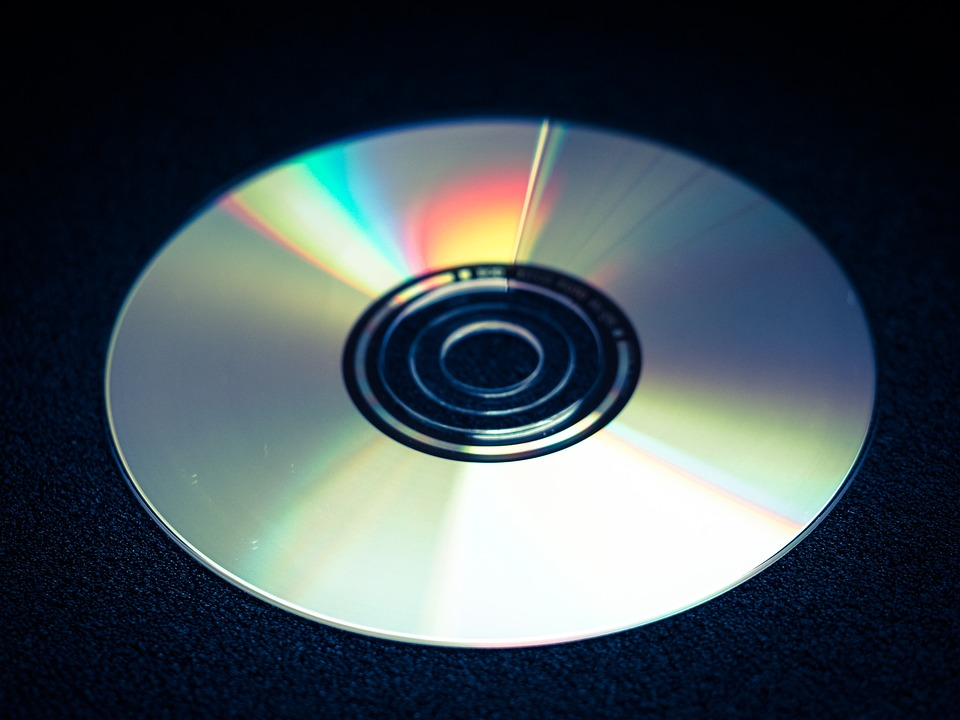
\includegraphics[width=\textwidth]{dvd.jpg}
\caption{This is in fact a DVD.}
\end{figure}
\end{column}
\end{columns}
\end{center}

\end{frame}

\section{Table}
\begin{frame}
\frametitle{Table}
\begin{table}
\begin{tabular}{l | c | c | c | c }
Competitor Name & Swim & Cycle & Run & Total \\
\hline
John T & 13:04 & 24:15 & 18:34 & 55:53 \\ 
Norman P & 8:00 & 22:45 & 23:02 & 53:47\\
Alex K & 14:00 & 28:00 & n/a & n/a\\
Sarah H & 9:22 & 21:10 & 24:03 & 54:35 
\end{tabular}
\caption{Triathlon results}
\end{table}

\end{frame}

\section{Code}
\subsection{C/C++ code}
\begin{frame}[fragile]
\frametitle{C/C++ code}

This is an example of C code.

\begin{cplusplus}
#include <stdio.h>

int main() {
    printf("Hello, world!\n");

    return 0;
}
\end{cplusplus}

\end{frame}

\subsection{Python code}
\begin{frame}[fragile]
\frametitle{Python code}

This is an example of Python code.
\begin{python}
import numpy as np


def matrix_product(m1, m2):
    return np.matmul(m1, m2)


m1 = np.array([[1, 0], [0, 1]])
m2 = np.array([[4, 1], [2, 2]]
prod = matrix_product(m1, m2)
\end{python}


\end{frame}

\section{Conclusion}
\begin{frame}
\frametitle{Conclusion}

This is the conclusion of the presentation!

\end{frame}

\begin{frame}[allowframebreaks, plain, noframenumbering]{References}
    \nocite{*}
    \bibliographystyle{plain}
    \bibliography{ref.bib}
\end{frame}

\begin{frame}[plain, noframenumbering]
    \begin{minipage}{\linewidth}
    \begin{tikzpicture}[remember picture, overlay]
        \fill[dvdPrimary] (current page.north east) rectangle ([yshift=3cm]current page.south west);
        \node[anchor=west] at (-1, -1) {\fontsize{90}{1} \selectfont \color{colorBackground} Thanks};
        \node[anchor=east] at (15, -5) {\small \color{dvdPrimary} made with \LaTeX\ and beamer};
    \end{tikzpicture}
    \end{minipage}
\end{frame}

\end{document}

